\documentclass[12pt]{article}
%\usepackage[portuguese]{babel}
\usepackage[utf8]{inputenc}
\usepackage[usenames,dvipsnames]{color}
\usepackage{setspace}
\usepackage{amsmath}
\usepackage{amsfonts}
\usepackage{amssymb}
\usepackage{mathtools}
\usepackage[top=3cm, bottom=2cm, left=3cm, right=2cm]{geometry}
\usepackage{tikz}
\usepackage{indentfirst}
\usepackage{algorithm} % algorithms
\usepackage{algpseudocode} % algorithms
\usepackage{textcomp}
\title{Relatorio IC}

% packages added by Marcelo
%
\usepackage{lscape}    % for landscape pages
\usepackage{hyperref}  % to allow hyperlinks
\usepackage{booktabs}  % nicer table borders
\usepackage{subfigure} % add subfigures

\graphicspath{{./figures/}} 

\definecolor{myblue}{RGB}{80,80,160}
\definecolor{mygreen}{RGB}{80,160,80}
\setstretch{1.5}

\begin{document}

\begin{center}
{\Large Stochastic U-Curve Branch and Bound \\}
\bigskip
{\bf Student:} \href{mailto:estrela.gustavo.matos@gmail.com}{Gustavo Estrela de Matos} \\
        {\bf Advisor:} \href{mailto:ulisses@ece.tamu.edu}{Dr. Ulisses Braga-Neto}
\end{center}

\section{Input Generation}
To generate the input for the problem we created two functions. The first creates a vector of floating points that simulates the values of a chain of a boolean lattice that respects the U-Curve assumption; and the second one adds a random noise to the values of the vector.

\subsection{Chain Generation}
The chain is generated based on a polynomial of second degree with positive leading coefficient. This polynomial has the minimum value of $0.1$ evaluated at some point $x^* \in [0, 1]$ which is determined by the user. The algorithm receives two arguments: the first one, $n$, represents the size of the chain; and the second one, $center \in [0, 1]$, specifies where is the minimum of the polynom. After creating a random polynom that holds our constraints, we split the $[0,1]$ interval in $n$ equaly spaced points, and evaluate the polynomial at these points, generating the curve.

\begin{algorithm}[t]
\caption{U-Curve Input Creator}
\begin{algorithmic}[1]
\Procedure{GeneratePoints}{$n, max\_distance, center$}
    \State $points \gets \{0, ..., 0\}$
    \State $p.a \gets random ()$
    \State $p.b \gets -2 * p.a * center$
    \State $p.c = (p.a^2 - 0.1) / (4 * p.a)$
    \State $dx \gets 1 / n$
    \State $x \gets 0$
    \For {$i \in \{0, ..., n\}$}
        \State $points_i \gets p (x)$
        \State $x \gets x + dx$
    \EndFor
    \State $j \gets n * random ()$
    \State $plain\_size \gets (n - j) * random ()$
    \For {$k \in \{1, ..., plain\_size\}$} \Comment Creates a plain area in the chain
        \State $points[j + k] \gets points[j]$
    \EndFor
    \State
    \Return $points$
\EndProcedure
\end{algorithmic}
\end{algorithm}

\subsection{Noise}
The noise is applied to the vector created by $GeneratePoints$, by adding that is in the interval 
$[-\alpha \frac{curve\_amplitude}{n}, \alpha \frac{curve\_amplitude}{n}]$, where $curve\_amplitude = max(v) - min (v)$ and $\alpha$ is a random variable with gaussian distribution with mean $0$ and standard deviation $\sigma$.

\begin{figure}[H]
\caption{Example of a curve generated with $\sigma = 0$}
\centering
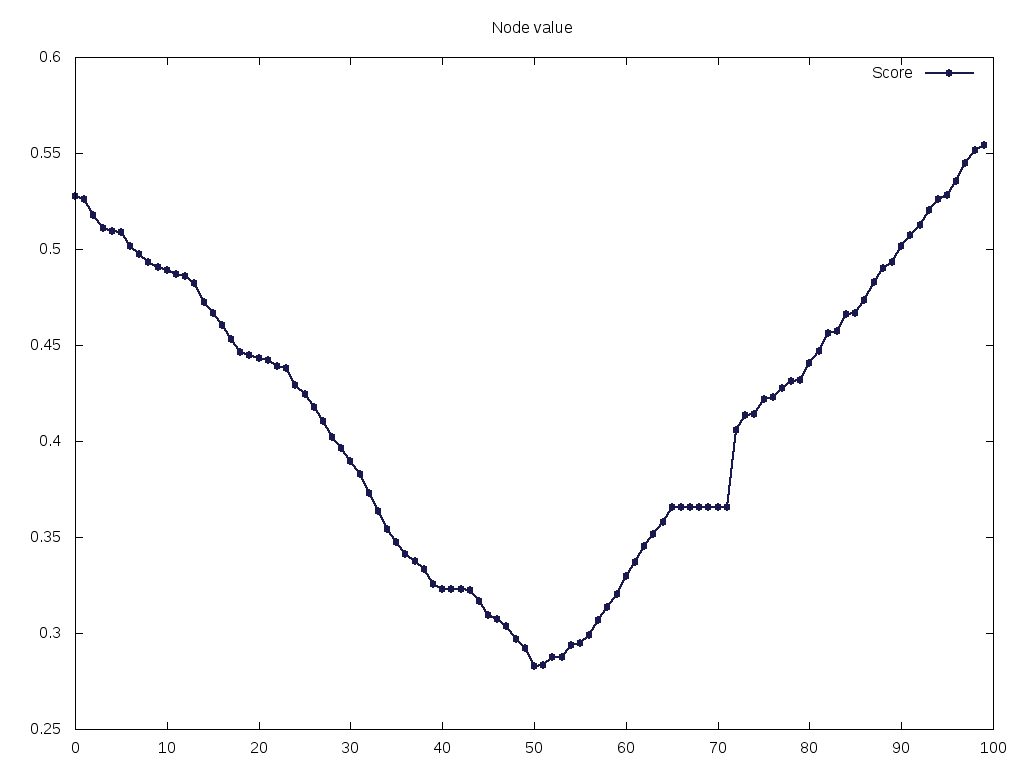
\includegraphics[scale=.5]{curve_sigma0}
\end{figure}

\begin{figure}[H]
\caption{Example of a curve generated with $\sigma = 1$}
\centering
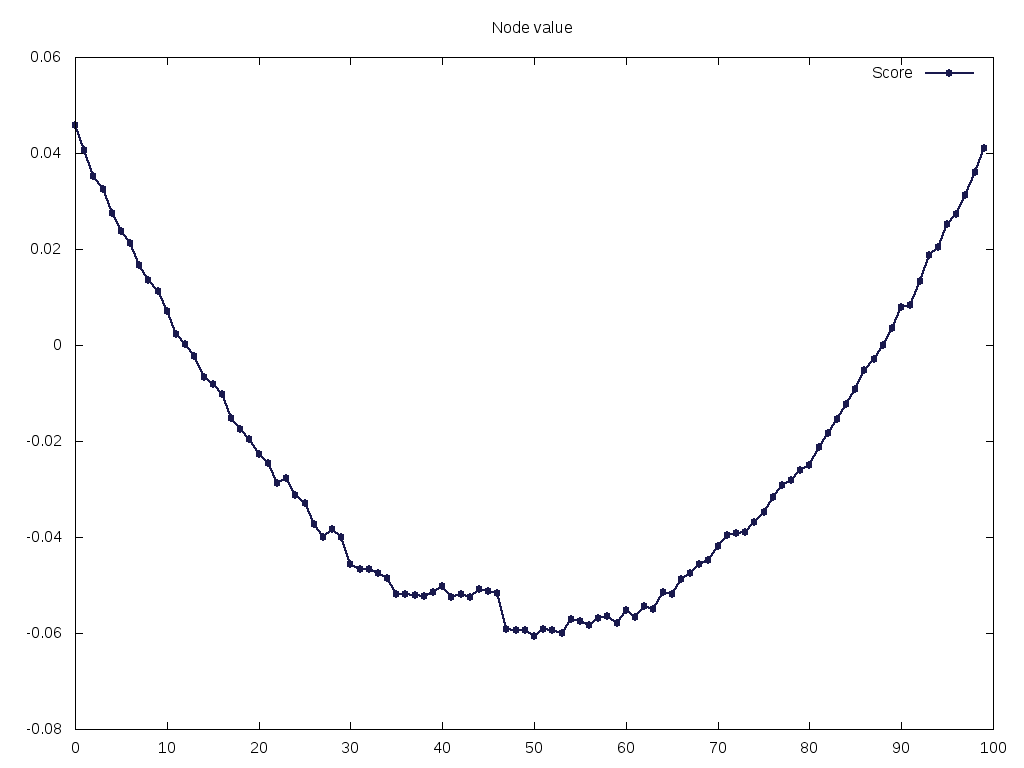
\includegraphics[scale=.5]{curve_sigma1}
\end{figure}

\begin{figure}[H]
\caption{Example of a curve generated with $\sigma = 2$}
\centering
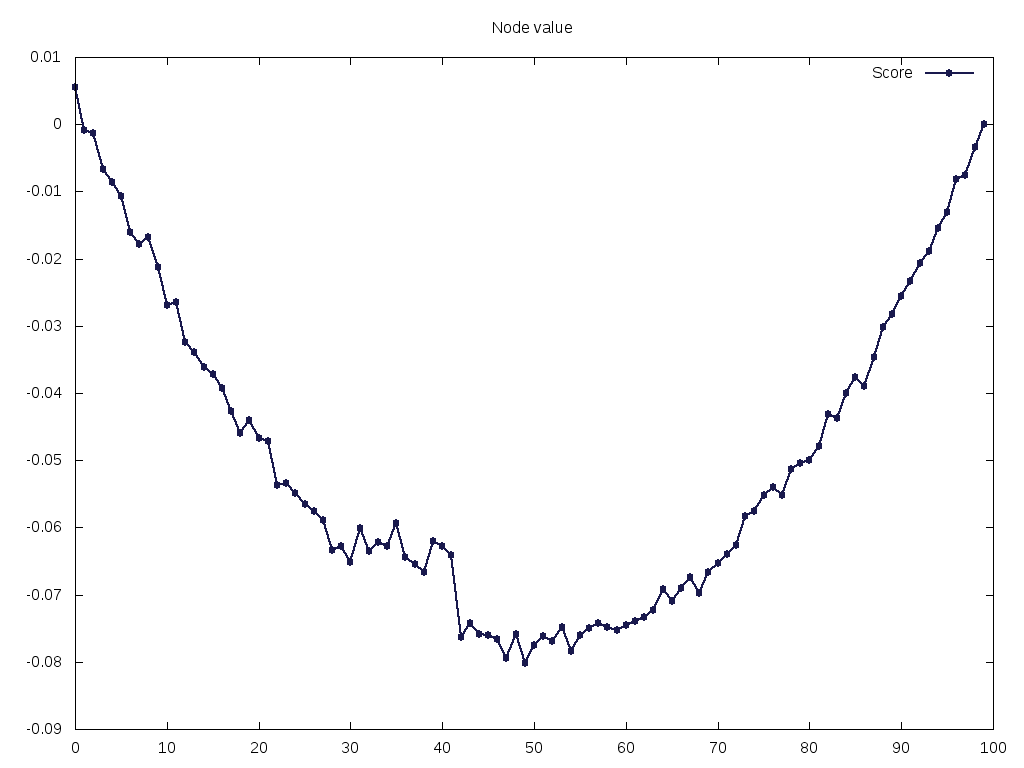
\includegraphics[scale=.5]{curve_sigma2}
\end{figure}

\newpage
\section{Bisection Algorithms}
\subsection{Traditional Bisection}
This is the simplest bisection algorithm we implemented. The basic idea of this algorithm is to divide the original problem in two halfs and, by analysing the neighbours of the node in the middle, determine which half has the minimum and then solve this half recursively. To guarantee the optimally of the algorithm (when the input respects the U-Curve assumption) we solve both halfs when the neighbours can't determine if the minimum lies to the left or right of the middle point.
\begin{algorithm}[h]
\caption{}
\begin{algorithmic}[1]
\Procedure{Bisection}{$v$}
    \State $n \gets v.length$
    \State $i \gets n / 2$
    \If {$(valley (v, i))$}
        \State
        \Return $v[i]$
    \Else
        \State $direction \gets SelectSide (v, i)$
        \If {$direction = Left$}
            \State
            \Return $Bisection ([v_i, ..., v_n])$
        \ElsIf {$direction = Right$}
            \State
            \Return $Bisection ([v_0, ..., v_{i - 1}])$
        \Else \Comment Unknown direction
            \State
            \Return $min (Bisection ([v_0, ..., v_{i - 1}]), Bisection ([v_i, ..., v_n]))$
        \EndIf
    \EndIf

\EndProcedure
\end{algorithmic}
\end{algorithm}

\begin{algorithm}[h]
\caption{}
\begin{algorithmic}[1]
\Procedure{SelectSide}{$v, i$}
    \State $d = v[i + 1] - v[i - 1]$
    \If {$|d| < \epsilon$}
        \State
        \Return Unknown
    \ElsIf {$d > 0$}
        \State
        \Return Left
    \Else
        \State
        \Return Right
    \EndIf
\EndProcedure
\end{algorithmic}
\end{algorithm}

\subsection {Mid-neighbour Bisection}
As an attempt to minimize the effects of noise in the traditional bisection algorithm we developed the Mid-neighbour Bisection, which brings two new ideas to the traditional bisection, that changes the evaluated points and also how we divide the problem in smaller problems.

The first idea consists in changing the points that are evaluated to decide which side to go. Instead of looking to the neighbours of the middle point, we now evaluate the points that are in the middle of the left half and right half. After evaluating these points, we calculate the difference between the left-middle point and middle point and also the difference between the right-middle point and the middle point to get two abstract slopes that can guarantee us which fraction of the input has the minimum value. 

The second idea considers the "reliabillity" of the abstract slopes mentioned before, for instance, if we say that the left slope (middle point - left-middle point) is negative, it's more likely that the function is going to increase from the left-middle point and before if the distance between these two points is greater. That happens because if the function decreases from the left-middle point and before, then the left-middle point suffered some noise that caused a peak (an inverted u-shape) and, considering that the points should describe a u-shape that would imply in a bigger noise for bigger distances of middle point and lef-middle point. We modeled the "reliability" of the abstract slope as a linear function that decreases from one to zero in $lg n$ steps.

The abstracts slopes are reduced to three different cases: 1 for growing, -1 for decreasing and 0 for plain areas or unreliable difference. Since we have three different slopes, there are nine different cases that need to be handled by the algorithm. Suppose that we are using the mid-neighbour bisection on a vector $v = \{v_1, ..., v_n\}$ and the right-middle, middle and left-middle point are, respectively, $lm, m, $ and $rm$. Then, the following pictures represent how the algorithm finds the minimum recursively.

    \begin{figure}[H]
        \centering
        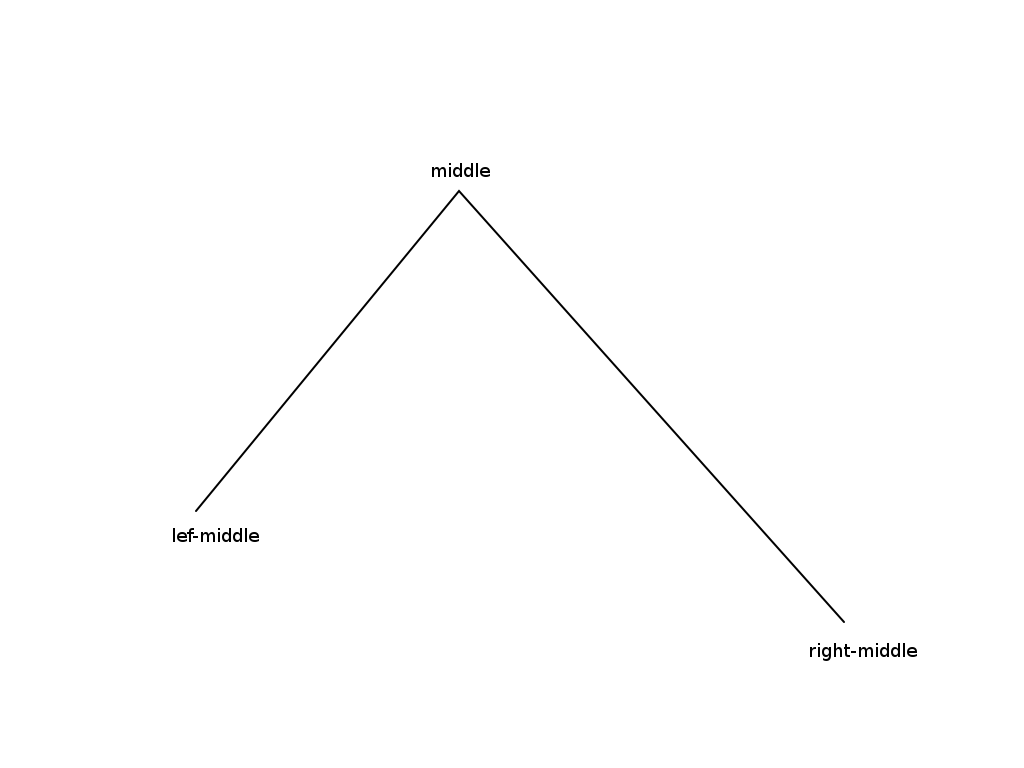
\includegraphics[scale=.35]{mid_case1}
        \caption{In this case we split the original problem into the two problem of finding the minimum of $\{v_1,..., v_{m - 1}\}$ and $\{v_m, ..., v_n\}$.}
    \end{figure}
    \begin{figure}[H]
        \centering
        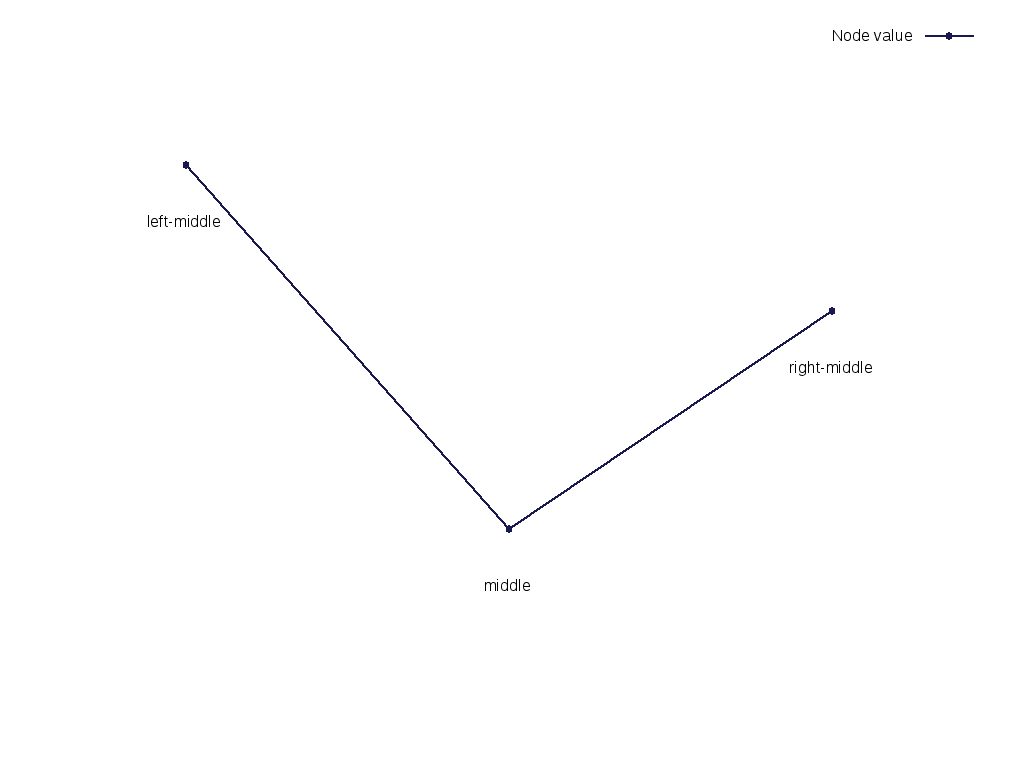
\includegraphics[scale=.35]{mid_case2}
        \caption{In this case we reduce the problem to finding the minimum of $\{v_{lm}, ..., v_{rm}\}$.}
    \end{figure}
    \begin{figure}[H]
        \centering
        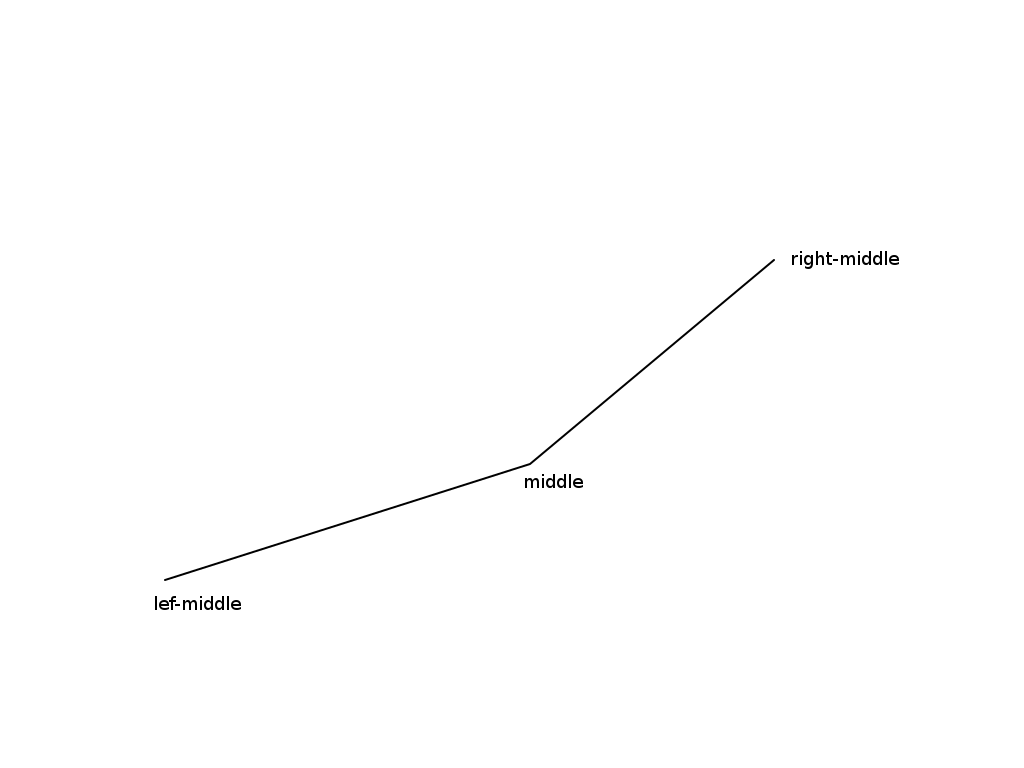
\includegraphics[scale=.35]{mid_case3}
        \caption{For this case we reduce the problem to finding the minimum of $\{v_1, ..., v_{m}\}$.}
    \end{figure}
    \begin{figure}[H]
        \centering
        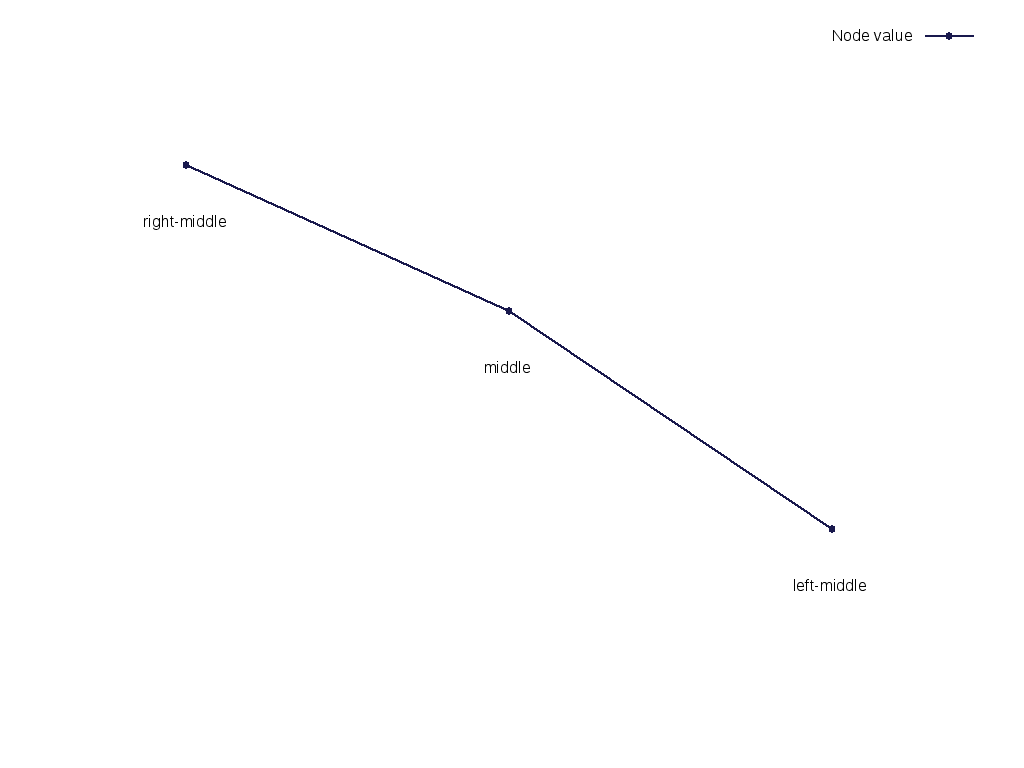
\includegraphics[scale=.35]{mid_case4}
        \caption{In this case we reduce the problem to finding the minimum of $\{v_m, ...v_n\}$.}
    \end{figure}
    \begin{figure}[H]
        \centering
        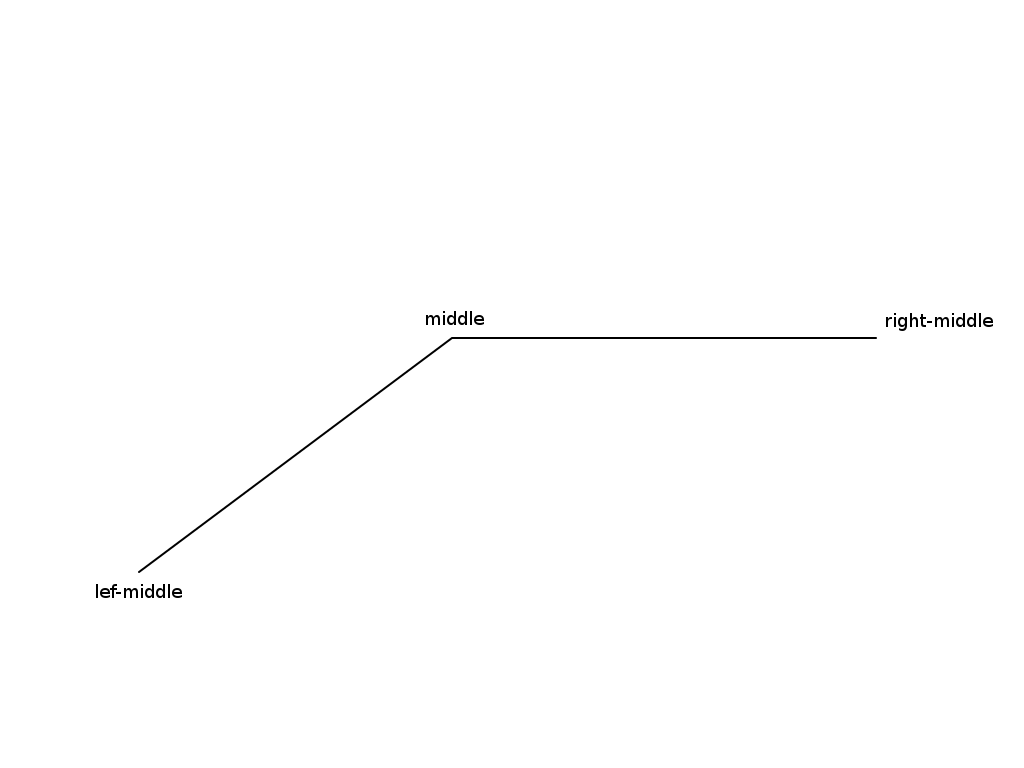
\includegraphics[scale=.35]{mid_case5}
        \caption{For this case we reduce the problem to finding the minimum of $\{v_1, ..., v_m\}$.}
    \end{figure}
    \begin{figure}[H]
        \centering
        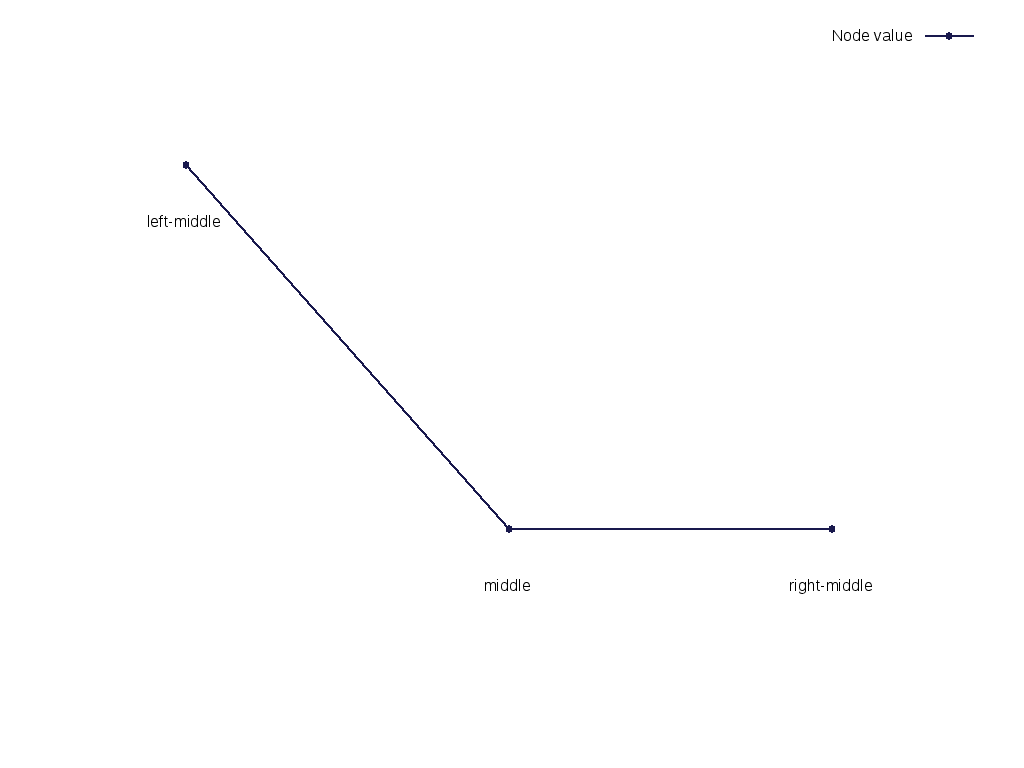
\includegraphics[scale=.35]{mid_case6}
        \caption{For this case we reduce the problem to finding the minimum of $\{v_{lm}, ..., v_m\}$.}
    \end{figure}
    \begin{figure}[H]
        \centering
        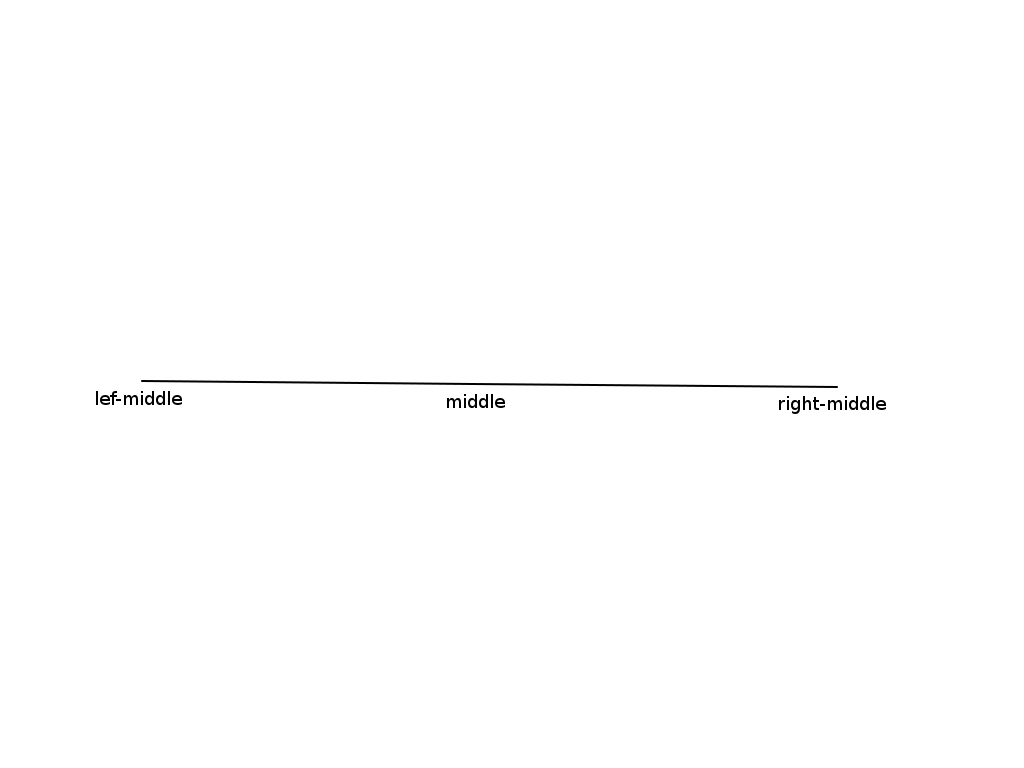
\includegraphics[scale=.35]{mid_case7}
        \caption{In this case we split the original problem into the two problem of finding the minimum of $\{v_1,..., v_{m - 1}\}$ and $\{v_m, ..., v_n\}$.}
    \end{figure}
    \begin{figure}[H]
        \centering
        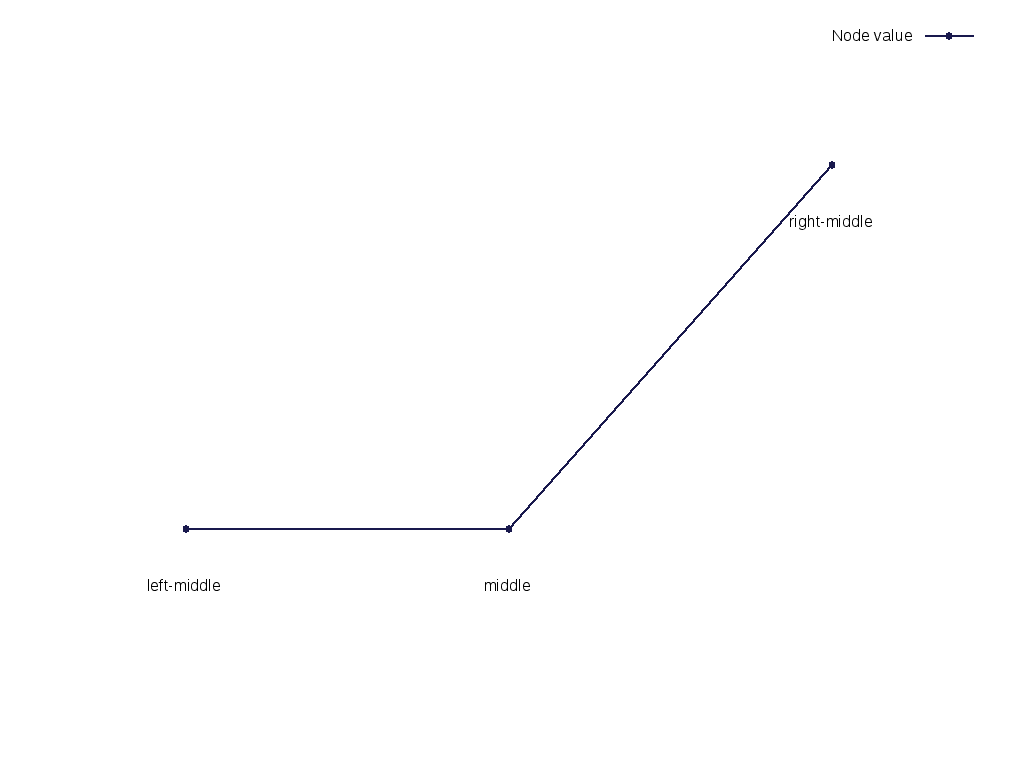
\includegraphics[scale=.35]{mid_case8}
        \caption{In this case we reduce the problem to finding the minimum of $\{v_1, ..., v_m\}$.}
    \end{figure}
    \begin{figure}[H]
        \centering
        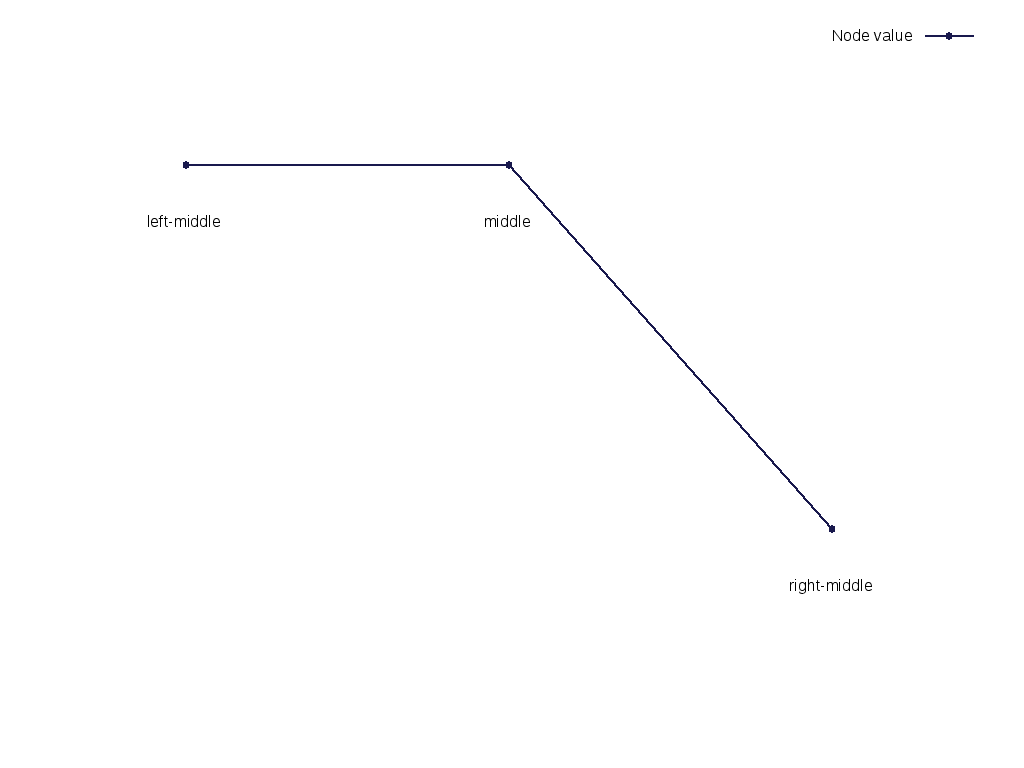
\includegraphics[scale=.35]{mid_case9}
        \caption{In this case we reduce the original problem to finding the minimum of $\{v_m, ..., v_n\}$}
    \end{figure}

\subsection{U-Curve Probabilistic Bisection}
The U-Curve Probabilistic Bisection (UPB) is a stochastic version of the algorithm we called "Traditional Bisection". The UPB algorithm keeps a probability mass function $f_i (x)$, for every iteration $i$ and every node $x$ of the search space, that can represent the algorithm belief, on iteration $i$, that the node $x$ is the answer to the problem. This algorithm has two key points: selecting the node to be evaluated and updating the probability mass function.

Different from the Traditional Bisection, we don't select the element that is the middle of the input to evaluate, instead we select the $m$-th element of the input vector $v$ such that:
\begin{equation*}
    m = \min\limits_{1 \leq i \leq n} \{i \mid f (v_i) \geq \frac{1}{2}\}.
\end{equation*}
, i.e the median of the possible solutions. The algorithm then compares the adjacent nodes of $v_m$ and decides which side the solution should be the same way it was done in the traditional bisection.


We call $p_c$ the probability that we chose the correct side when evaluating $v_m$'s neighbours and $\alpha = \sum_{j = 1}^m f_i (v_j)$. In the case where the actual solution lies in the right side of $v_m$, the probability mass function update is calculated by:
\begin{flalign*}
    f_{i + 1} (y) &=
    \begin{cases}
        (\frac{1}{1 - \alpha})p_cf_i (y) \textup{ if } y \geq v_m \\
        \alpha (1 - p_c) f_i (y) \textup{ if } y < v_m
    \end{cases}
\end{flalign*}
. This update is similar for the case when the solution lies in the left side of $v_m$. If there is no defined value for $f_0$, we simply assume that the probability of being a solution is distributed uniformily between all nodes of the chain.

The algorithm terminates when the first quantile or when the third quantile, of the possible solutions, are the same node as the second quantile (median), which is the solution given by the algorithm. This termination condition avoids an early termination, that would be caused by a local minimal element if we used the same termination condition as we did in the traditional bisection.
\begin{algorithm}[h]
\caption{}
\begin{algorithmic}[1]
\Procedure{UPB}{$v, pmf$}
    \State $n \gets v.length$
    \State $Quantiles \gets FindQuantiles (pmf)$
    \While {$Quantiles_1 \neq Quantiles_2 \textbf{ and } Quantiles_2 \neq Quantiles_3$}
        \State $direction \gets SelectSide (v, i)$
        \If {direction is Unknown} \Comment Unknown direction
            \State
            \Return $SplitUPB (v, pmf, Quantile_2)$
        \Else
        \State $UpdatePMF (pmf, Quantile_2, F (Quantile_2), direction)$
        \EndIf
    \State $Quantiles \gets FindQuantiles (pmf)$
    \EndWhile
    \State
    \Return $Quantile_2$
\EndProcedure
\end{algorithmic}
\end{algorithm}


\subsection{Mid-neighbour Probabilistic Bisection}
The Mid-neighbour Probabilistic Bisection (MPB) is a probabilistic algorithm that partitionates the search space into four different parts and, according to the value of the points between the subsets, decides in which portion of the chain the minimum should be. The partition on the chain is made according to the quantiles of the $pmf$ and the points we evaluate are $v_{lm}$, $v_{m}$ and $v_{rm}$, which we define as:
\begin{itemize}
    \item{$lm = \min\limits_{1 \leq i \leq n} \{i \mid f (v_i) \geq \frac{1}{4}\}$.}
    \item{$m = \min\limits_{1 \leq i \leq n} \{i \mid f (v_i) \geq \frac{2}{4}\}$.}
    \item{$rm = \min\limits_{1 \leq i \leq n} \{i \mid f (v_i) \geq \frac{3}{4}\}$.}
\end{itemize}

After finding the points $v_{lm}$, $v_m$ and $v_{rm}$ we calculate the cost $c$ of these points and update the $pmf$ according to the following rules:
\begin{itemize}
    \item{If $c (v_{rm}) - c (v_{lm}) > \epsilon:$} then we guess that the minimum should be to the left of $v_{rm}$.
    \item{If $c (v_{rm}) - c (v_{lm}) < -\epsilon:$} then we guess that the minimum should be to the right of $v_{lm}$.
    \item{If $|c (v_{rm}) - c (v_{lm})| < \epsilon$ and $v_m < {min (v_{rm}, v_{lm})}:$} then we guess that the minimum should be between $v_{lm}$ and $v_{rm}$
    \item{If $|c (v_{rm}) - c (v_{lm})| < \epsilon$ and $v_m \geq {min (v_{rm}, v_{lm})}:$} then we can't guess where the minimum is. To overcome this, we divide the problem in the node $v_m$ so we can solve, recursively, two problems and return the minimum of the two solutions.
\end{itemize}

\begin{algorithm}[h]
\caption{}
\begin{algorithmic}[1]
\Procedure{MPB}{$v, pmf$}
    \State $n \gets v.length$
    \State $Quantiles \gets FindQuantiles (pmf)$
    \State $v_{lm} \gets Quatile_1$
    \State $v_{m} \gets Quatile_2$
    \State $v_{rm} \gets Quatile_3$
    \While {$v_{lm} \neq v_m \textbf{ and } v_{rm} \neq v_m$}
        \State $d \gets c (v_{rm}) - c (v_{lm})$
        \If {$abs (d) < \epsilon$}
            \If {$v_m < min (v_{rm}, v_{lm})$}
                \State $UpdatePMF (pmf, v_{lm}, F (v_{lm}), Right)$
                \State $UpdatePMF (pmf, v_{rm}, F (v_{lm}), Left)$
             \Else \Comment Unknown direction
                \State
                \Return $SplitMPB (v, pmf, v_m)$
            \EndIf
            \ElsIf {$d > \epsilon$}
                \State $UpdatePMF (pmf, v_{rm}, F (v_{rm}), Left)$
            \Else
                \State $UpdatePMF (omf, v_{lm}, F (v_{lm}), Right)$
        \EndIf
        \State $Quantiles \gets FindQuantiles (pmf)$
        \State $v_{lm} \gets Quatile_1$
        \State $v_{m} \gets Quatile_2$
        \State $v_{rm} \gets Quatile_3$
    \EndWhile
    \State
    \Return $v_m$
\EndProcedure
\end{algorithmic}
\end{algorithm}



\section{Results}
\begin{figure}[H]
        \centering
        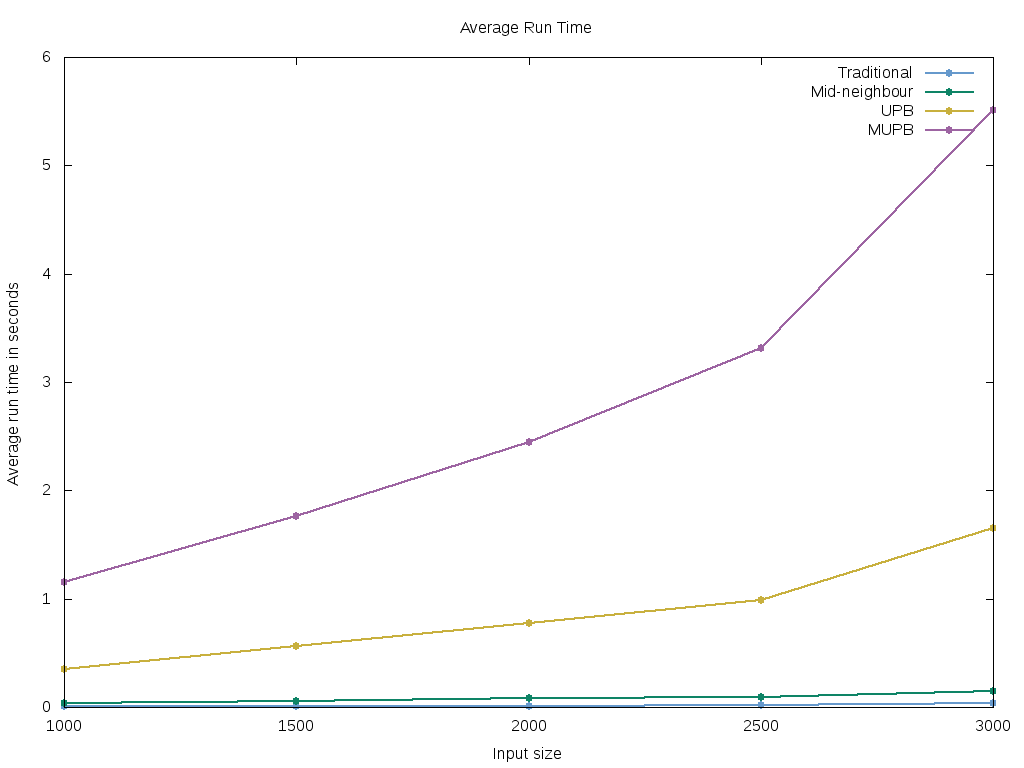
\includegraphics[scale=.5]{time_plot_result}
\end{figure}
\begin{figure}[H]
        \centering
        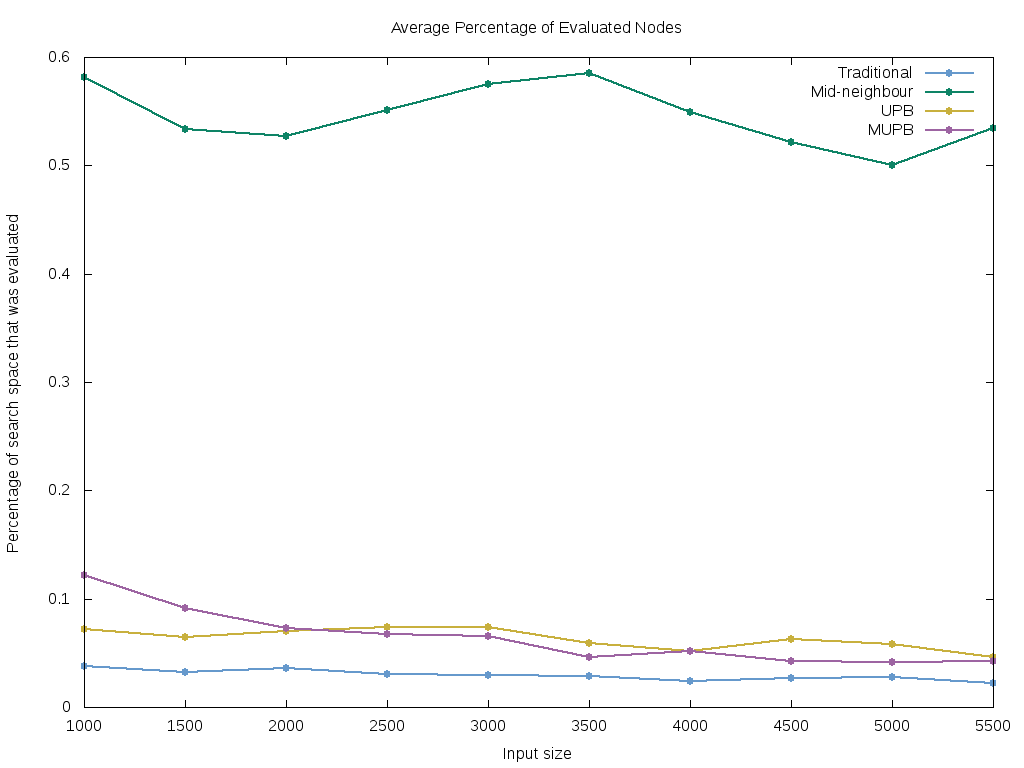
\includegraphics[scale=.5]{evaluations_plot_result}
\end{figure}
\begin{figure}[H]
        \centering
        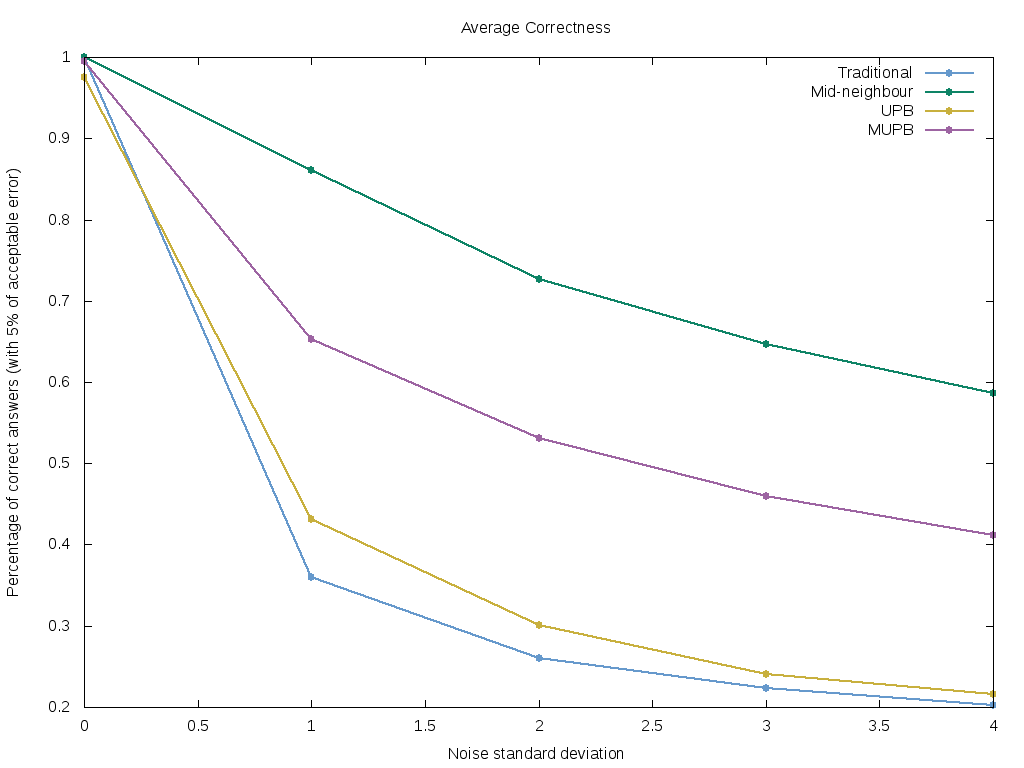
\includegraphics[scale=.5]{correctness_plot_result}
\end{figure}
\begin{figure}[H]
        \centering
        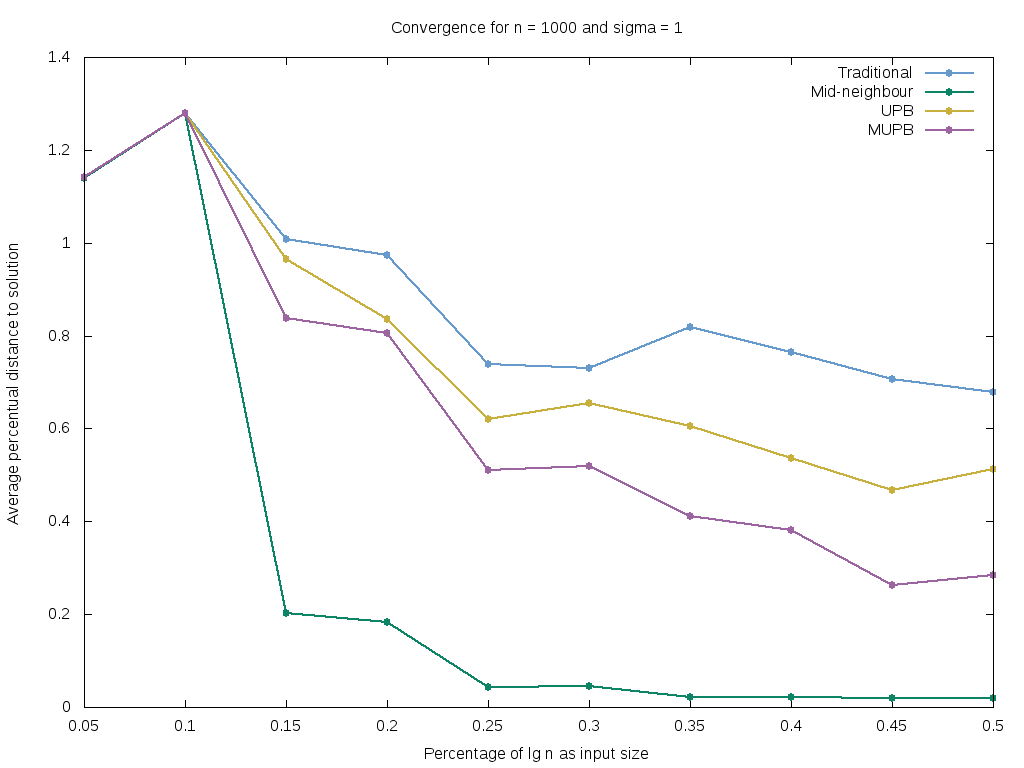
\includegraphics[scale=.5]{convergence_plot_n1000_s1}
\end{figure}

\begin{figure}[H]
    \centering
    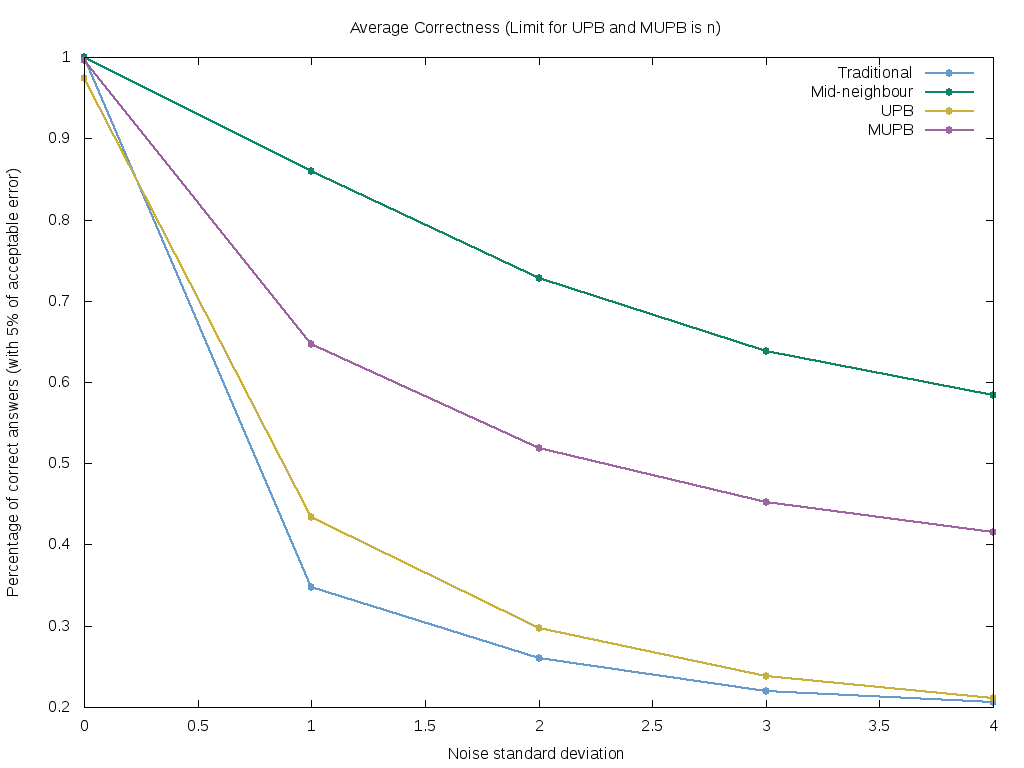
\includegraphics[scale=.5]{correctness_plot_ln}
\end{figure}

\begin{figure}[H]
    \centering
    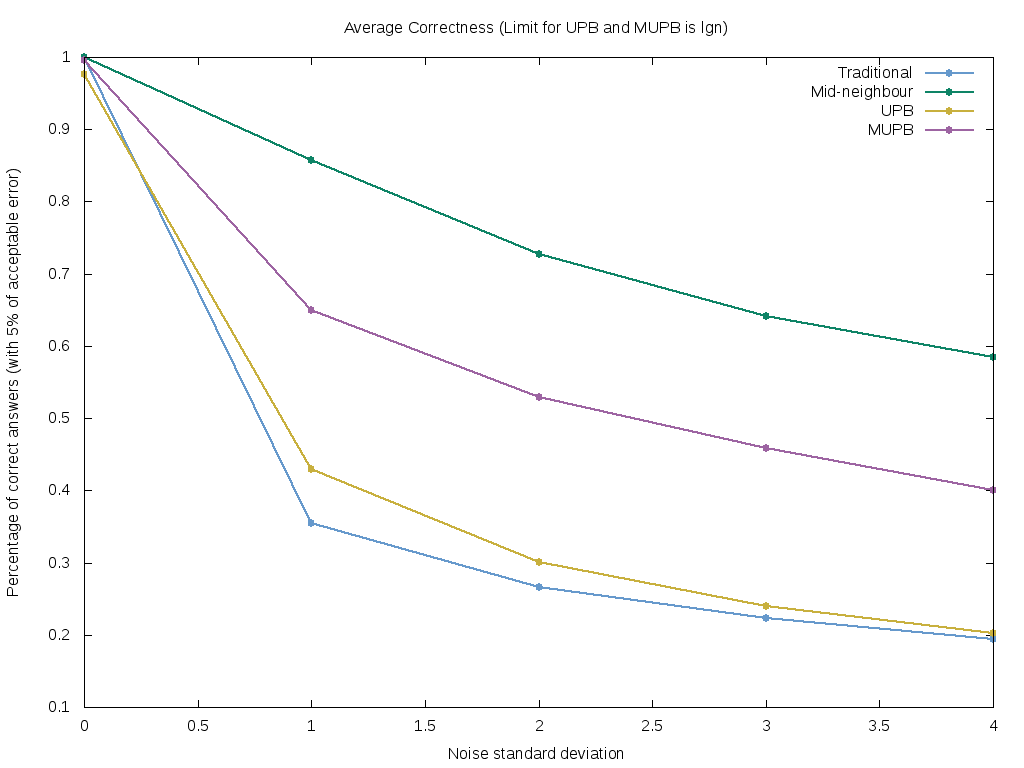
\includegraphics[scale=.5]{correctness_plot_lgn}
\end{figure}

\end{document}

